\documentclass[tikz,border=7pt]{standalone}
\usepackage{palatino}
\usepackage{amsmath}
\usepackage[none]{hyphenat}
\usepackage{xcolor}
\usetikzlibrary{arrows.meta,calc}

\definecolor{mapink}{HTML}{20252B}
\definecolor{mapgray}{HTML}{707780}
\definecolor{mapline}{HTML}{9199A1}
\definecolor{mapblue}{HTML}{0072B2}
\definecolor{mapbluefill}{HTML}{EAF3FA}
\definecolor{mapgreen}{HTML}{18857A}
\definecolor{mapgreenfill}{HTML}{E9F4F1}
\definecolor{mapred}{HTML}{D55E00}

\begin{document}
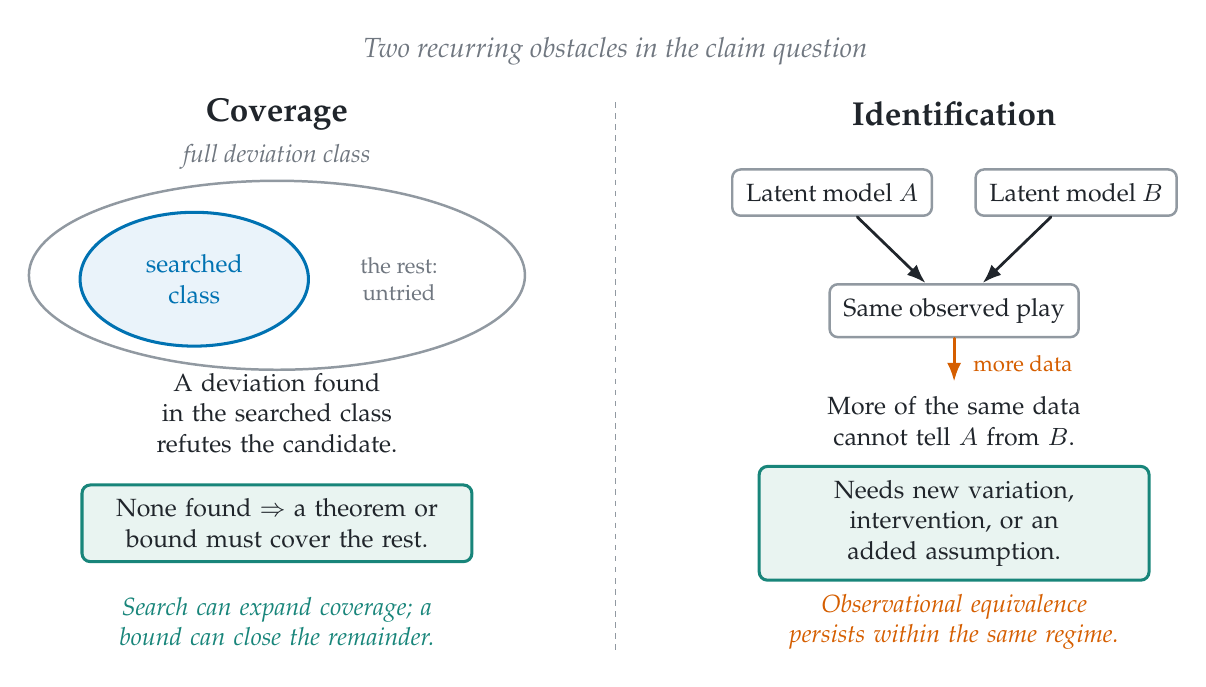
\begin{tikzpicture}[
  font=\rmfamily,
  box/.style={draw=mapline, fill=white, text=mapink, line width=0.9pt,
    rounded corners=3pt, align=center, font=\rmfamily\small, inner sep=5pt},
  greenbox/.style={draw=mapgreen, fill=mapgreenfill, text=mapink, line width=1.1pt,
    rounded corners=3pt, align=center, font=\rmfamily\small, inner sep=5pt,
    text width=4.6cm},
  flow/.style={draw=mapink, line width=1.0pt, -{Latex[length=2.4mm,width=1.8mm]}, line cap=round},
  block/.style={draw=mapred, line width=1.1pt, -{Latex[length=2.4mm,width=1.8mm]}, line cap=round},
  ptitle/.style={font=\rmfamily\bfseries\large, text=mapink},
  stmt/.style={align=center, font=\rmfamily\small, text=mapink, text width=4.8cm},
  note/.style={align=center, font=\rmfamily\small\itshape},
]

% ===== shared header =====
\node[font=\rmfamily\itshape, text=mapgray] at (0,4.15) {Two recurring obstacles in the claim question};

% ===== divider =====
\draw[mapline, line width=0.5pt, dash pattern=on 2pt off 2pt] (0,3.5) -- (0,-3.5);

% =========================================================
% LEFT PANEL: COVERAGE
% =========================================================
\node[ptitle] at (-4.3,3.35) {Coverage};

% nested sets
\node[note, text=mapgray] at (-4.3,2.80) {full deviation class};
\draw[draw=mapline, line width=0.9pt] (-4.3,1.30) ellipse (3.15 and 1.20);
\fill[mapbluefill] (-5.35,1.25) ellipse (1.45 and 0.85);
\draw[draw=mapblue, line width=1.1pt] (-5.35,1.25) ellipse (1.45 and 0.85);
\node[align=center, font=\rmfamily\small, text=mapblue] at (-5.35,1.25) {searched\\class};
\node[align=center, font=\rmfamily\footnotesize, text=mapgray] at (-2.75,1.25) {the rest:\\untried};

% outcomes
\node[stmt] at (-4.3,-0.45) {A deviation found in the searched class refutes the candidate.};
\node[greenbox] at (-4.3,-1.85) {None found $\Rightarrow$ a theorem or bound must cover the rest.};

% takeaway
\node[note, text=mapgreen, text width=5.0cm] at (-4.3,-3.1)
  {Search can expand coverage; a bound can close the remainder.};

% =========================================================
% RIGHT PANEL: IDENTIFICATION
% =========================================================
\node[ptitle] at (4.3,3.35) {Identification};

\node[box] (mA) at (2.75,2.35) {Latent model $A$};
\node[box] (mB) at (5.85,2.35) {Latent model $B$};
\node[box, text=mapink] (data) at (4.3,0.85) {Same observed play};
\draw[flow] (mA) -- (data);
\draw[flow] (mB) -- (data);

% more data does not help
\draw[block] (data.south) -- ++(0,-0.55);
\node[font=\rmfamily\footnotesize, text=mapred, right=2pt] at ($(data.south)+(0.05,-0.32)$) {more data};
\node[stmt, text width=4.8cm] at (4.3,-0.55) {More of the same data cannot tell $A$ from $B$.};

\node[greenbox] at (4.3,-1.85) {Needs new variation, intervention, or an added assumption.};

\node[note, text=mapred, text width=5.0cm] at (4.3,-3.1)
  {Observational equivalence persists within the same regime.};

\end{tikzpicture}
\end{document}
